\documentclass{article}
\usepackage{graphicx}
\graphicspath{ {images/} }
\usepackage[utf8]{inputenc}

\title{Autómata Finito Determinístico De Todas Las Palabras Reservadas De ANSI C}
\author{Leon Tejeda 2CM5}
\date{Octubre 2020}

\begin{document}
\maketitle
Se realizo el grafo de un autómata finito determinístico de todas las palabras reservadas de ANSI C
Para esto encontrmos que las palabras reservadas eran.

\centering
\begin{tabular}{c c}
auto		&	int \\
break		&	long \\
case		&	register \\
char		&	return \\
const		&	short \\
continue	&	signed \\
default	&	sizeof \\
do		&	static \\
double	&	struct \\
else		&	switch \\
enum		&	typedef \\
extern	&	union \\
float		&	unsigned \\
for		&	void \\
goto		&	volatile \\
if		&	while \\
\end{tabular}


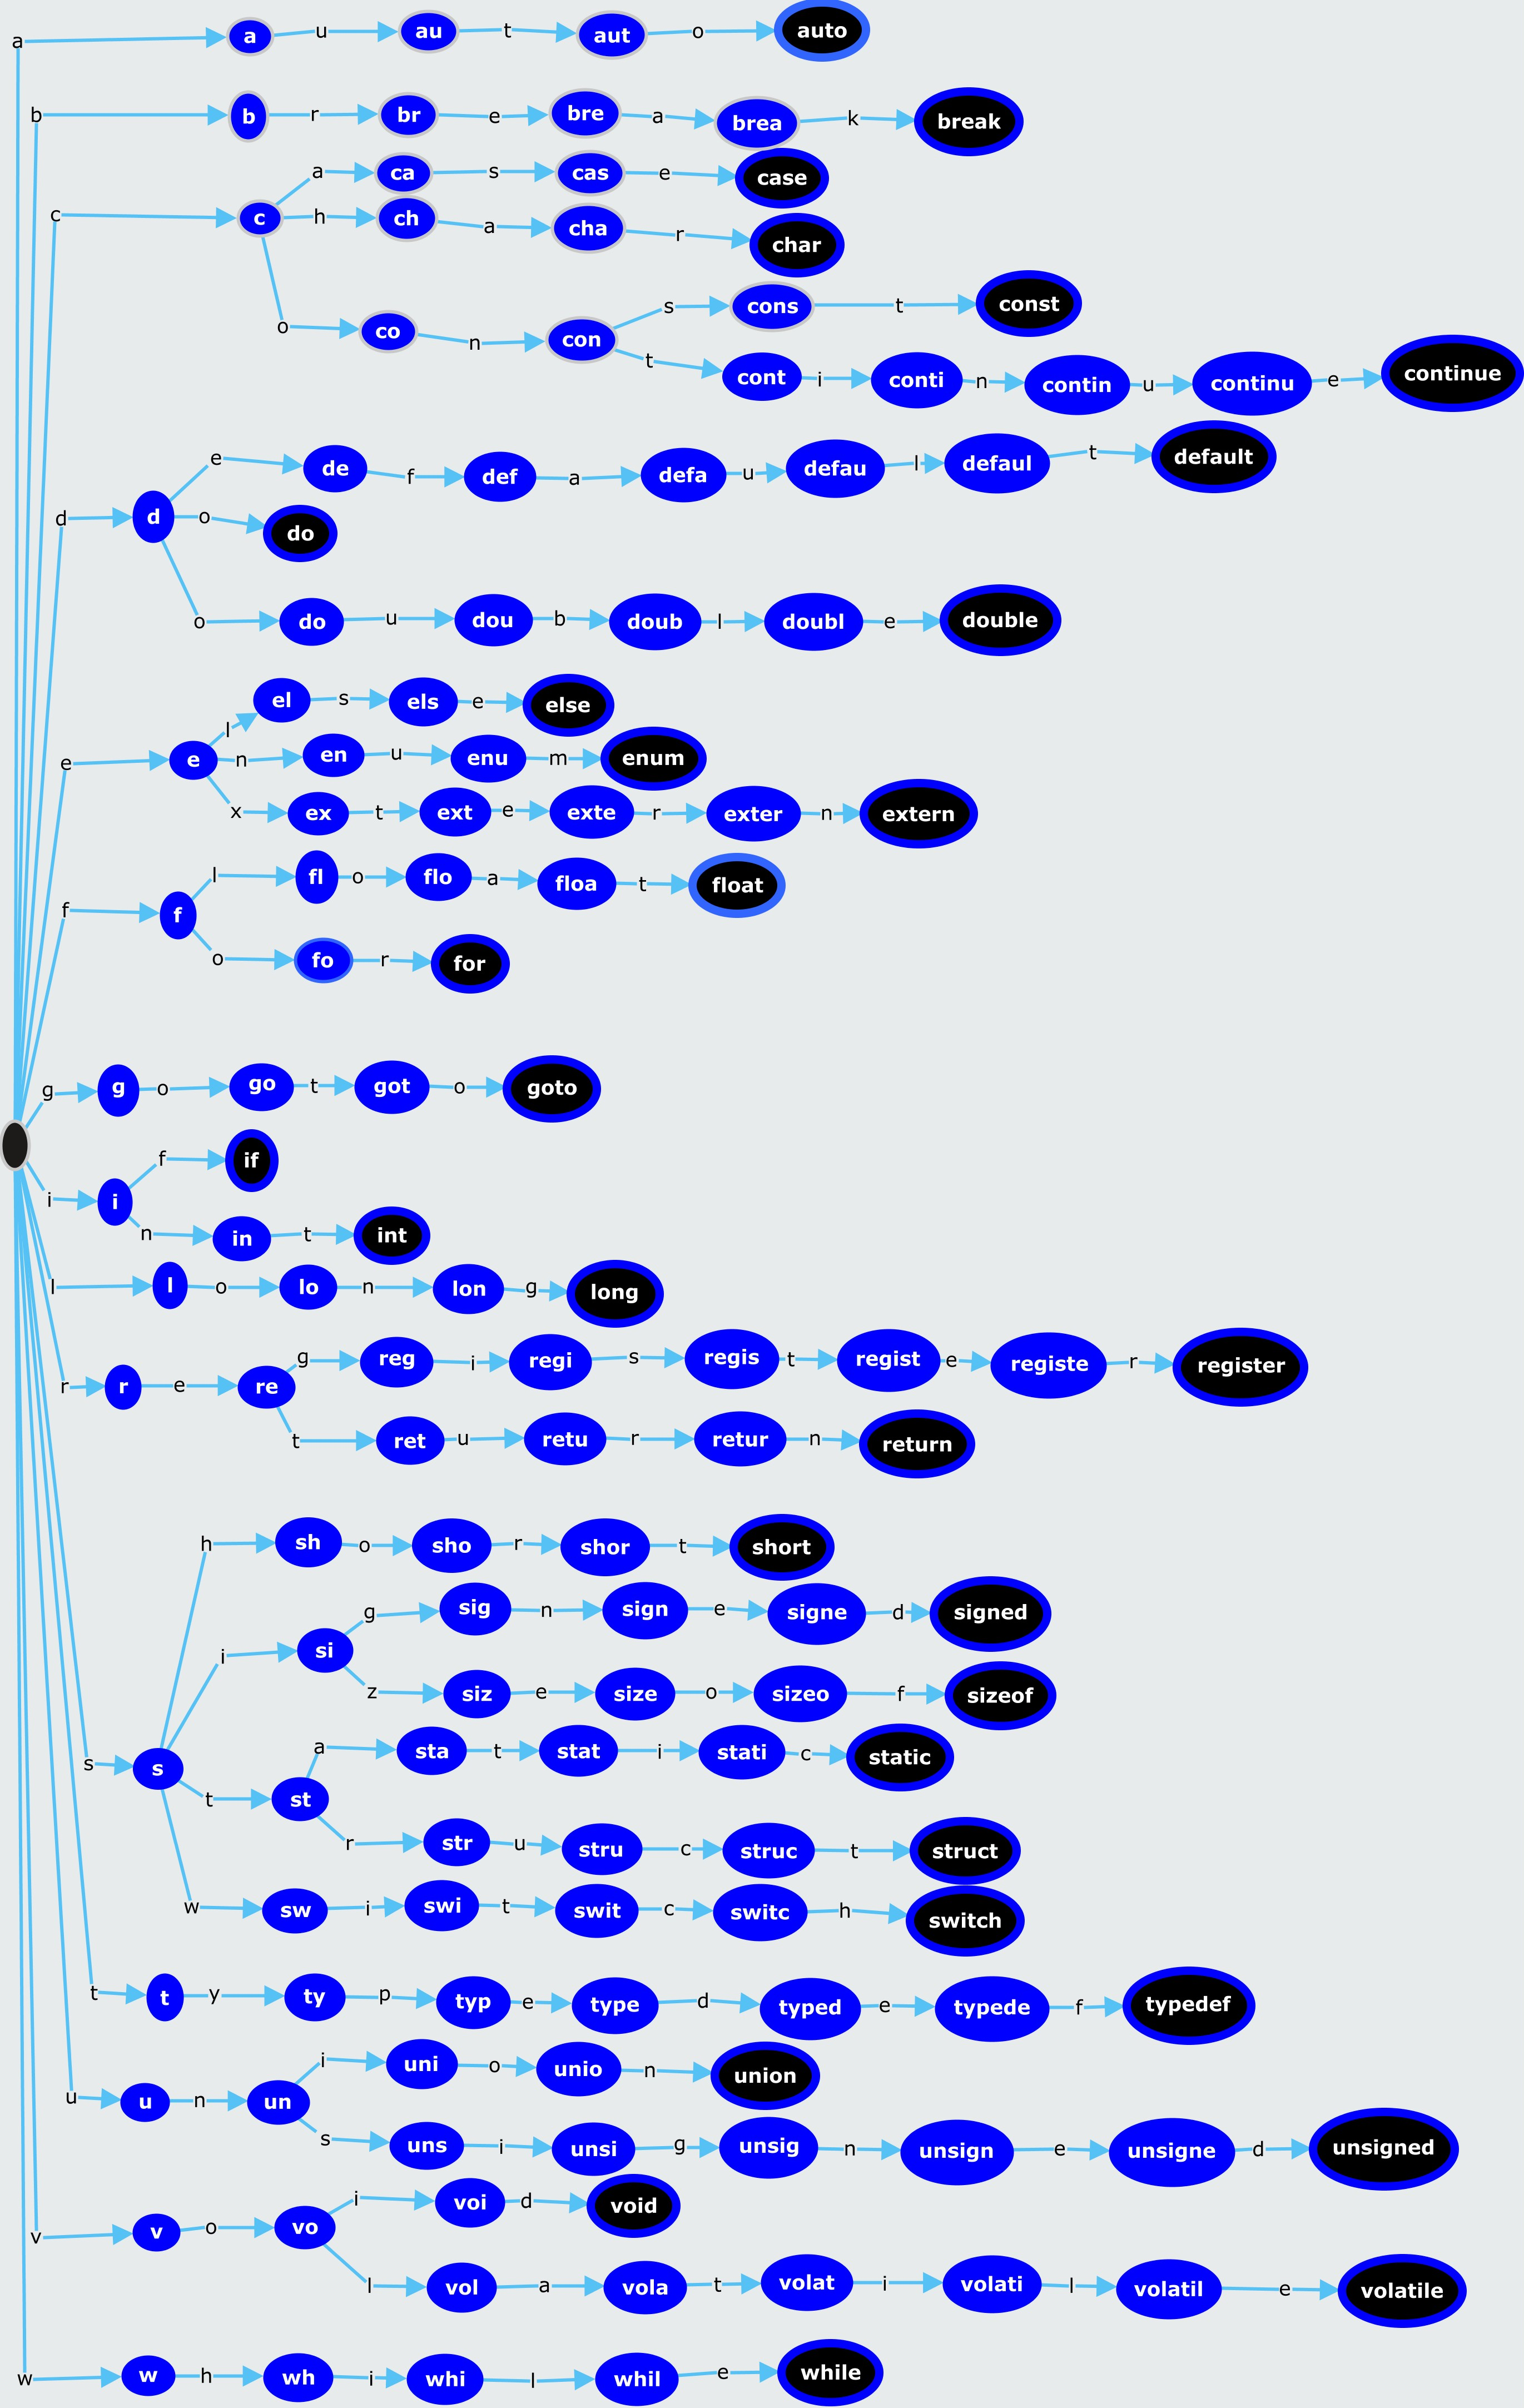
\includegraphics[width= 15cm, height= 20cm]{Grafo.jpg}
\end{document}